\documentclass[a4paper,10pt]{article}
\usepackage[T1]{fontenc}
\usepackage[utf8]{inputenc}
\usepackage[english]{babel}
\usepackage{lmodern}
\usepackage[top=1.6cm,bottom=1.8cm,left=1.9cm,right=1.9cm]{geometry}
\usepackage{titlesec,enumitem,xcolor,graphicx,lastpage,fancyhdr}
\usepackage{fontawesome5}
\usepackage[hidelinks]{hyperref}

\hypersetup{colorlinks=true,urlcolor=blue!70!black,linkcolor=blue!70!black}
\pagestyle{fancy}\fancyhf{}\renewcommand{\headrulewidth}{0pt}
\fancyfoot[C]{\small\color{gray}Page \thepage\ of \pageref{LastPage}}
\setlength{\parindent}{0pt}

\titleformat{\section}{\large\bfseries\color{blue!70!black}}{}{0em}{}[\vspace{-0.7em}\rule{\textwidth}{0.5pt}]
\titlespacing{\section}{0pt}{9pt}{5pt}
\setlist[itemize]{leftmargin=1.1em,itemsep=2pt,topsep=2pt,parsep=0pt}
\newcommand{\role}[4]{\vspace{3pt}\noindent\hspace{0.6em}\parbox[t]{0.38\textwidth}{\raggedright\textbf{#1}}\hfill\parbox[t]{0.58\textwidth}{\raggedleft\textit{#2}}\\{\textit{#3}\hfill\textit{#4}}\vspace{1pt}}

\begin{document}
\noindent
\begin{minipage}[t]{0.78\textwidth}
\vspace{0pt}
{\huge\bfseries Prabhavit Gupta}\\[8pt]
{\small \faPhone\ +39-351-610-7807 \quad \faEnvelope\ \href{mailto:prabhavitg@gmail.com}{prabhavitg@gmail.com} \quad \faLinkedin\ \href{https://www.linkedin.com/in/prabhavit/}{Linkedin} \quad \faMapMarker*\ Venice, Italy}
\end{minipage}\hfill
\begin{minipage}[t]{0.18\textwidth}
\vspace{0pt}\raggedleft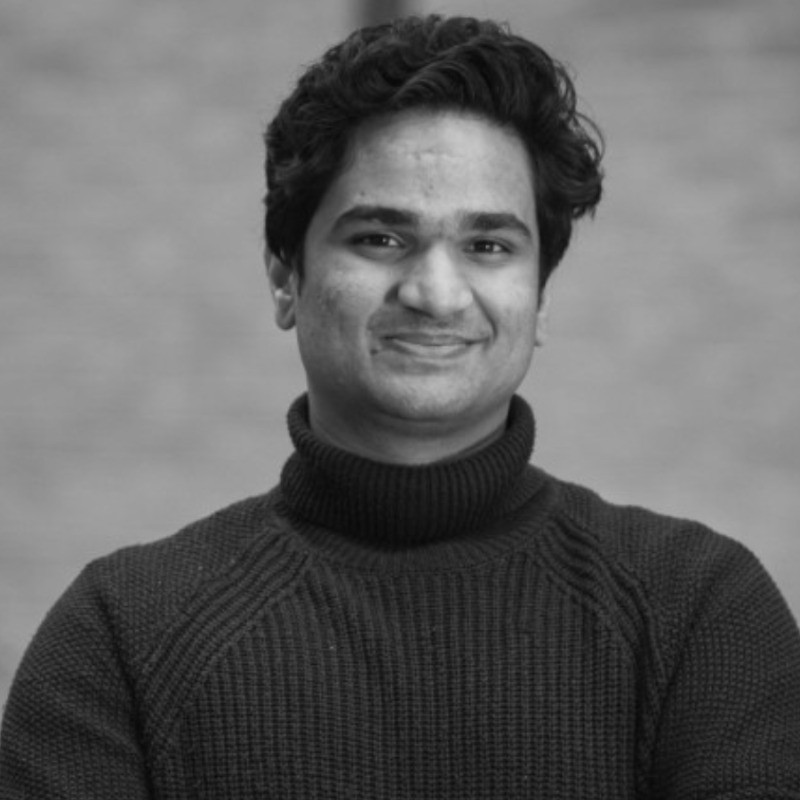
\includegraphics[width=2.3cm,height=2.3cm,keepaspectratio]{photo.jpg}
\end{minipage}

\section{Career Summary}
\begin{itemize}
\item Automation Engineer with dual degrees in Mechanical and Management Engineering (Politecnico di Milano), experienced in automated machinery, process control, and systems integration.
\item Solid foundation in industrial automation, PLC/HMI logic, hardware-in-the-loop testing, and field commissioning for regulated production lines.
\item Proven record of writing diagnostic test suites, coordinating technical validation on customer sites, and ensuring high reliability across packaging and industrial workflows.
\end{itemize}

\section{Technical Skills}
\begin{itemize}
\item \textbf{Industrial Automation} -- PLC Programming Logic, HMI Interfaces, Automated Packaging Lines, Commissioning \& Collaudo, Sensor Integration
\item \textbf{Engineering \& Quality} -- Mechanical Systems Design, Quality Assurance, Pharma \& Medical Packaging Standards, Technical Support
\item \textbf{Software \& Scripting} -- Python, C++, Bash, SQL, Git, Linux, Automated Test Suites
\item \textbf{Protocols \& Controls} -- Modbus, Industrial Ethernet, REST APIs, Documentation, Root Cause Analysis
\end{itemize}

\section{Visa \& Language}
\begin{itemize}
\item \textbf{Language} -- Italian (Conversational / Intermediate), English (Fluent / Professional), Hindi (Native)
\item \textbf{Work Authorization} -- European Long Term Residence Permit - No Sponsorship required. Driving License (Patente B).
\end{itemize}

\section{Professional Experience}
\role{\href{https://flowspace.co}{FlowSpace.co}}{Automation Lead Developer (Full time, Freelance)}{London, UK}{Mar 2024 -- Ongoing}
\begin{itemize}
\item \textbf{Automation \& Systems Engineering:}
\begin{itemize}[label=--]
\item Designed automated process monitoring pipelines and integration test harnesses, verifying operational parameters across production services.
\item Developed real-time telemetry loggers and exception handling routines to detect hardware/software synchronization anomalies.
\item Authored technical commissioning documentation, system operating procedures, and diagnostic guidelines for field engineers.
\end{itemize}
\item \textbf{Quality Assurance \& Operations:}
\begin{itemize}[label=--]
\item Supervised continuous system upgrades, maintaining 99.9\% availability across core automated platforms.
\item Executed comprehensive validation runs, analyzing error logs and coordinating with hardware vendors for prompt issue remediation.
\end{itemize}
\item \textit{Tools: Python, Linux, Bash, Automated Testing, REST APIs, Docker, Git, Jira}
\end{itemize}

\role{Urlink}{Systems Automation Engineer}{Milan, Italy}{Jul 2023 -- Feb 2024}
\begin{itemize}
\item Engineered automated verification scripts to validate data acquisition from connected industrial machinery and field sensors.
\item Assisted engineering teams during system acceptance testing (collaudo) and customer site deployment routines.
\item Documented equipment specifications, interface protocols, and troubleshooting procedures for client technical staff.
\end{itemize}

\role{UltraStrategy}{Automation Developer}{Remote, Germany}{Sep 2022 -- Jun 2023}
\begin{itemize}
\item Built automated data collection scripts monitoring machinery performance and throughput metrics across manufacturing sites.
\item Automated routine diagnostic checks and generated structured compliance reports for quality audits.
\end{itemize}

\section{Education}
\role{Politecnico di Milano}{M.Sc. in Management Engineering (Digital Business \& ICT)}{Milan, Italy}{2020 -- 2023}
\role{Thapar Institute of Engineering and Technology}{B.E. in Mechanical Engineering}{Punjab, India}{2014 -- 2018}

\end{document}
